\section{Разработка TLA+ спецификации алгоритма Raft}

В рамках технологической части была разработана формальная
спецификация алгоритма консенсуса Raft на языке TLA+. Спецификация
используется для описания поведения кластера в терминах состояний,
переходов и сообщений, а также служит основой для последующей
модельной проверки и интеграции с системой верификации соответствия
спецификации и программной реализации.

\subsection{Формальная спецификация алгоритма}

Разработанная TLA+ спецификация описывает основные механизмы
алгоритма консенсуса Raft в терминах состояний узлов, обмена
сообщениями и допустимых переходов системы. Полный текст
спецификации приведён в приложении~Б.

В спецификации заданы константы, определяющие состав кластера,
множество возможных значений, роли узлов, типы сообщений и
параметры, ограничивающие пространство состояний при модельной
проверке. Такое описание позволяет отделить логику протокола от
конкретной конфигурации модели и использовать одну и ту же
спецификацию для различных наборов параметров.

Состояние системы задаётся глобальной переменной сообщений и набором
локальных переменных каждого сервера. К глобальному состоянию
относится мультимножество сообщений, находящихся в сети. Локальные
переменные описывают текущий срок узла, его роль, отданный голос,
содержимое журнала, индекс фиксации, множество полученных голосов,
а также параметры репликации журнала, включая индексы
синхронизации с последователями и признак ожидания ответа на
предыдущий запрос. Дополнительно используются вспомогательные
переменные, ограничивающие число выборов и перезапусков, а также
отображение подтверждённых значений, применяемое при формулировке
инвариантов.

В спецификации определён набор вспомогательных функций,
используемых для вычисления кворума, определения характеристик
журнала, а также моделирования отправки, дублирования, удаления и
обработки сообщений. Эти функции не задают самостоятельных
переходов системы, а служат для компактного и однозначного
описания действий алгоритма.

Начальное состояние кластера задаётся оператором инициализации
$Init$. В нём все серверы находятся в состоянии последователей,
имеют начальный срок, пустые журналы и отсутствие сообщений в
сети. Такое состояние соответствует стандартному начальному
условию для запуска протокола Raft.

Динамика системы задаётся через действия, объединённые в оператор
$Next$. В спецификации отражены основные переходы алгоритма:
инициация выборов лидера, отправка и обработка сообщений
$RequestVote$ и $AppendEntries$, переход кандидата в состояние
лидера, продвижение индекса фиксации, обновление срока при
получении более нового сообщения, а также обработка ответов
последователей. Тем самым спецификация охватывает как механизм
выбора лидера, так и механизм репликации журнала.

Полная спецификация задаётся в стандартной для TLA+ форме как
сочетание оператора инициализации и отношения переходов:
начальное состояние определяется формулой $Init$, а дальнейшее
поведение системы --- формулой $[][Next]_{vars}$.

\subsection{Тестирование модели}

Проверка разработанной TLA+ спецификации выполнялась с помощью средства TLC,
которое исследует достижимые состояния модели и контролирует выполнение
заданных свойств безопасности. В рамках проверки рассматривались два
инварианта, отражающие ключевые требования к корректности алгоритма Raft.

Первый инвариант, \texttt{NoLogDivergence}, выражает согласованность
зафиксированной части журналов. Его смысл состоит в том, что если у двух
серверов некоторый индекс уже входит в зафиксированный префикс журнала, то
записи по всем индексам этого общего префикса должны совпадать. Тем самым
проверяется, что после фиксации команда не может иметь разные значения на
разных узлах кластера.

Второй инвариант, \texttt{LeaderHasAllAckedValues}, связывает состояние журнала
лидера с подтверждёнными клиенту значениями. Если некоторое значение помечено
как подтверждённое, то любой актуальный лидер обязан содержать его в своём
журнале. Это свойство важно с точки зрения сохранности уже подтверждённых
данных и исключает ситуацию, при которой новый лидер утрачивает значение, о
подтверждении которого уже было сообщено клиенту.

Результаты проверки представлены на рис.~\ref{fig:tla-09}. В рамках выбранной
конфигурации было исследовано более 36 тысяч состояний. Нарушений заданных
инвариантов обнаружено не было.

\begin{figure}
  \centering
  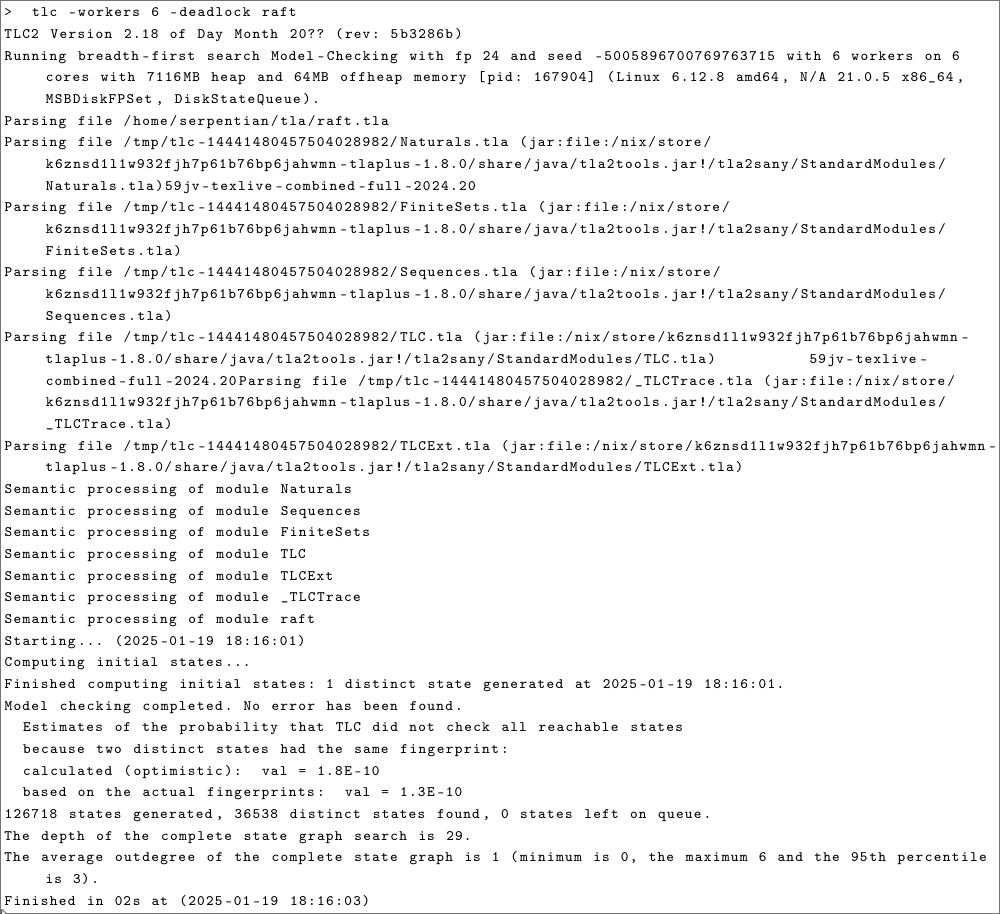
\includegraphics[scale=0.4]{inc/tla-09.png}
  \caption{Результаты проверки модели в TLC}
  \label{fig:tla-09}
\end{figure}

Таким образом, выполненная проверка модели показывает, что разработанная
спецификация сохраняет основные свойства безопасности Raft в пределах
исследованного пространства состояний и может использоваться далее как
формальная основа для сопоставления с программной реализацией.
